% This is the ADASS_template.tex LaTeX file, 24 Oct 2025.
% It is based on the ASP general author template file, but modified to reflect the specific
% requirements of the ADASS proceedings.

% This is the aspauthor.tex LaTeX file
% Copyright 2021, Astronomical Society of the Pacific Conference Series
% Revision:  29 November 2021

% To compile, at the command line positioned at this folder, type:
% pdflatex ADASS_template
% pdflatex ADASS_template
% This will create a file called ADASS_template.pdf

\documentclass[11pt,twoside]{article}

% Do NOT use ANY packages other than asp2023. 
\usepackage{asp2023}

\aspSuppressVolSlug
\resetcounters

% References must all use BibTeX entries in a .bibfile.
% References must be cited in the text using \citet{} or \citep{}.
% Do not use \cite{}.
% See ManuscriptInstructions.pdf for more details
\bibliographystyle{asp2021}

% The ``markboth'' line sets up the running heads for the paper.
% 1 author: "Surname"
% 2 authors: "Surname1 and Surname2"
% 3 authors: "Surname1, Surname2, and Surname3"
% >3 authors: "Surname1 et al."
% Replace ``Short Title'' with the actual paper title, shortened if necessary.
% Use mixed case type for the shortened title
% Ensure shortened title does not cause an overfull hbox LaTeX error
% See ASPmanual2010.pdf 2.1.4  and ManuscriptInstructions.pdf for more details
\markboth{Gheller et al.}{Scalable Segmentation with TUNA}


\begin{document}

\title{Scalable Deep-Learning Segmentation of Extended and Diffuse Radio Sources with TUNA}

% Note the position of the comma between the author name and the 
% affiliation number.
% Authors surnames should come after first names or initials, eg John Smith, or J. Smith.
% Author names should be separated by commas.
% The final author should be preceded by "and".
% Affiliations should not be repeated across multiple \affil commands. If several
% authors share an affiliation this should be in a single \affil which can then
% be referenced for several author names. If only one affiliation, no footnotes are needed.
% See ManuscriptInstructions.pdf and ASP's manual2010.pdf 3.1.4 for more details
\author{Claudio Gheller,$^1$ Nicoletta Sanvitale,$^1$
Alice Beccati,$^2$ and Franco Vazza,$^3$}
\affil{$^1$INAF - Institute for Radio Astronomy, Bologna, Italy; \email{claudio.gheller@inaf.it}}
\affil{$^2$Department of Computer Science and Engineering, University of Bologna, Bologna, Italy}
\affil{$^3$Department of Physics and Astronomy, University of Bologna, Bologna, Italy}

% This section is for ADS Processing.  There must be one line per author. paperauthor has 9 arguments.
\paperauthor{Claudio Gheller}{claudio.gheller@inaf.it}{}{INAF}{Institute for Radio Astronomy}{Bologna}{Bologna}{40129}{Italy}
\paperauthor{Nicoletta Sanvitale}{nicoletta.sanvitale@inaf.it}{}{INAF}{Institute for Radio Astronomy}{Bologna}{Bologna}{40129}{Italy}
\paperauthor{Alice Beccati}{alice.beccati@studio.unibo.it}{}{University of Bologna}{Department of Computer Science and Engineering}{Bologna}{Bologna}{40129}{Italy}
\paperauthor{Franco Vazza}{franco.vazza2@unibo.it}{}{University of Bologna}{Department of Physics and Astronomy}{Bologna}{Bologna}{40129}{Italy}

% There should be one \aindex line (commented out) for each author. These are used to
% build up the author index for the Proceedings. The surname must come first, followed by
% initials. Note the use of ~ before each initial to control spacing.
% The \author entries (see above) have surname last. These \aindex entries have
% surname first.
% The Aindex.py command willl create them for you after you have constructed the \author
% The first entry should be the first author, for bold-facing the author index page-reference

%\aindex{Gheller,~C.}
%\aindex{Sanvitale,~N.}
%\aindex{Beccati,~A.}
%\aindex{Vazza,~F.}


\begin{abstract}
Wide-area radio surveys require automated recovery of extended galaxies
and faint diffuse emission. We evaluate the segmentation quality and GPU
performance of TUNA, a convolutional--transformer segmentation network, on high-resolution LoTSS-DR2 images. TUNA identifies 1.76 million
connected detections, recovers 96.8\% of a reference radio-galaxy sample and
detects diffuse emission in 94.3\% of selected galaxy-cluster systems. We benchmark strong and weak GPU scaling and FP32, FP16 and BF16 training.
Two-GPU strong scaling and mixed-precision FP16 achieve speedups of
approximately $1.9\times$ and $1.98\times$, respectively, without appreciable
changes in test-set segmentation metrics. These results demonstrate the
importance of jointly optimizing numerical precision and GPU allocation.
\end{abstract}

% These lines show examples of subject index entries. At this stage these have to commented
% out, and need to be on separate lines. Eventually, they will be automatically uncommented
% and used to generate entries in the Subject Index at the end of the Proceedings volume.
% Don't leave these in! - replace them with ones relevant to your paper.
%\ssindex{FOOBAR!conference!ADASS 2019}
%\ssindex{FOOBAR!organisations!ASP}

% These lines show examples of ASCL index entries. At this stage these have to commented
% out, and need to be on separate lines. Eventually, they will be automatically uncommented
% and used to generate entries in the ASCL Index at the end of the Proceedings volume.
% The ascl.py command will scan your paper on possible code names.
% Don't leave these in! - replace them with ones relevant to your paper.
%\ooindex{FOOBAR, ascl:1101.010}


\section{Introduction}
The LOFAR Two-metre Sky Survey (LoTSS), operating at 120--168 MHz, provides
841 DR2 pointings at approximately 6 arcsec resolution
\citep{shimwell2022lofar}. These images contain compact sources, extended radio
galaxies and diffuse cluster emission whose irregular morphologies challenge
conventional source finders.

TUNA (TransUNet Network for radio Astronomy) was introduced to identify
low-surface-brightness radio emission \citep{Sanvitale2025} and subsequently
extended to jointly segment radio galaxies and diffuse cluster emission. Here, we assess its strong and weak GPU scaling and
the effects of reduced precision on training time and segmentation quality.

\section{Methodology}

\subsection{Segmentation network and training data}
TUNA combines a ResNet-50 feature extractor, a 12-layer Vision Transformer encoder and
a U-Net-like decoder \citep{chen2021transunet,Sanvitale2025}. It has approximately
105.9 million trainable parameters and uses equally weighted cross-entropy
and Dice losses.

The training data combine diffuse radio maps from numerical simulations
with observed LoTSS-DR2 radio-galaxy morphologies. A LOFAR-like eight-hour observation, including
thermal noise, deconvolution and primary-beam correction, is simulated with
WSClean \citep{offringa-wsclean-2014}.
Of 300 simulated fields, 250 form the development set and 50 the
independent test set. This yields approximately 4000 training and 800
test tiles of $512\times512$ pixels. The training runs use a 5\% validation
portion; model quality is compared on the unchanged test set. The reference model is trained for
100 epochs with batch size 24, initial learning rate 0.005 and polynomial
learning-rate decay. At inference, overlapping tiles are merged by retaining
the central $128\times128$ pixels to limit edge artefacts. The emission class
is evaluated through intersection-over-union (IoU), precision, recall and F1.

\subsection{Computational experiments}

Experiments were performed on the CINECA Leonardo Booster,  whose compute
nodes each provide four NVIDIA A100 GPUs with 64 GB of memory per GPU. Our TUNA implementation
was developed in PyTorch, and multi-GPU training was managed using Hugging
Face Accelerate with PyTorch Distributed Data Parallel. 
We consider two standard
data-parallel scaling regimes. In \emph{strong scaling}, the total workload and global batch size are held fixed as the GPU count increases from one to two and four. The speedup and parallel efficiency are
$S_N=T_1/T_N$ and $E_N^{\mathrm{strong}}=S_N/N$, respectively, where $T_N$ is the execution time for the same workload on $N$ GPUs. In \emph{weak scaling}, the batch size per GPU is held fixed while the global batch size grows in proportion to the GPU count (one, two, four, and eight GPUs). Runs using up to four GPUs were executed within one node, whereas the
eight-GPU weak-scaling run used two nodes. The weak-scaling efficiency is defined as $E_N^{\mathrm{weak}}=t_1/t_N$, where $t_N$ is the iteration time on $N$ GPUs.
Strong scaling used a fixed global batch size of 24, corresponding to local
batch sizes of 24, 12 and 6 on one, two and four GPUs. Weak scaling used a
fixed local batch size of 24, giving global batch sizes of 24, 48, 96 and 192.
These tests measure different limits of data-parallel training. 



Single-GPU experiments also compare FP32 with mixed-precision FP16 and BF16. Automatic mixed precision executes computationally intensive operations, such as convolutions and matrix multiplications, in reduced precision when numerically appropriate, while operations requiring greater numerical stability remain in FP32. Model parameters and accumulated gradient buffers remain in FP32. FP16 training employs gradient scaling to reduce gradient underflow, whereas BF16 generally does not require gradient scaling because of its wider dynamic range.
All experiments compare segmentation quality on held-out test data as
well as execution time. Each configuration was repeated four times, and results are reported as the
mean and standard deviation.

\section{Results}

%\subsection{Survey-scale segmentation}

Applied to LoTSS-DR2, TUNA yields 1756628 connected detections after
structures smaller than two synthesized beams are rejected. Of these,
498901 have a largest angular size (LAS) above 40 arcsec. TUNA recovers 26733 of
27623 independently catalogued extended and giant radio galaxies (96.78\%)
and diffuse emission in 83 of 88 selected galaxy-cluster systems (94.3\%). 
Components are not necessarily unique physical sources: neighbours
can merge and galaxies can fragment. Figure~\ref{fig:pointing} illustrates
the pointing-level segmentation and source detections. On an A100,
inference processes approximately 28 tiles per second, or a typical
LoTSS-DR2 pointing in about 30 s.

\begin{figure}[!htbp]
\centering
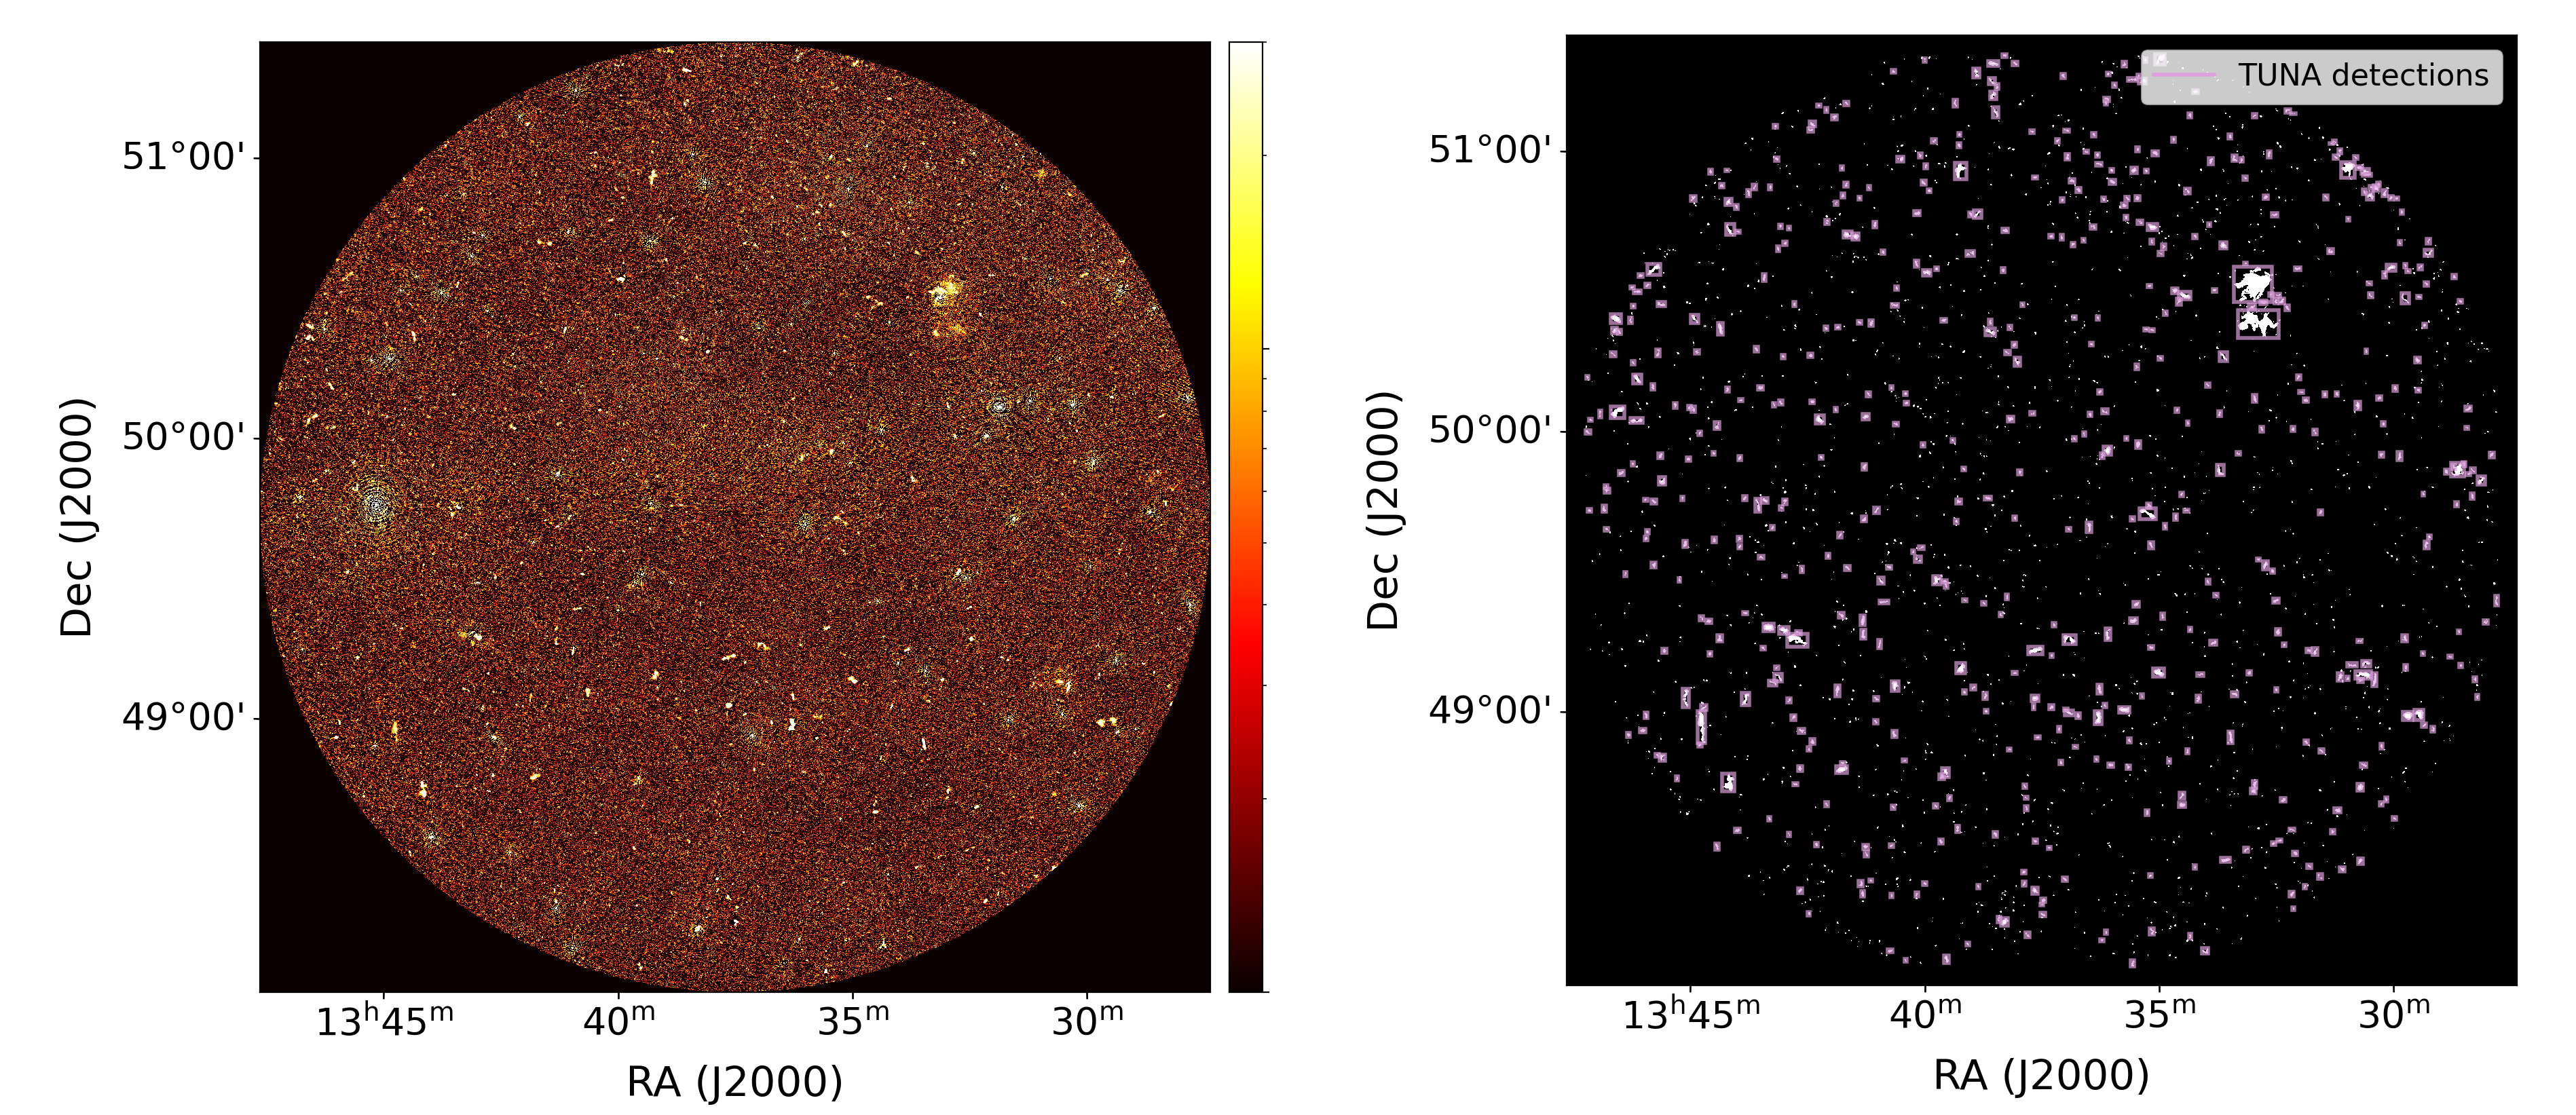
\includegraphics[width=0.9\linewidth]{ADASS26_C202_f1.png}
\caption{LoTSS-DR2 pointing P42Hetdex07: radio image (left) and TUNA
detections with LAS $>40$ arcsec (right).}
\label{fig:pointing}
\end{figure}


%\subsection{Strong and weak scaling}

Figure~\ref{fig:performance} summarizes the GPU benchmarks. For a fixed
training workload, adding a second GPU yields about 1.9$\times$ speedup
($\sim95\%$ efficiency), but four GPUs deliver only about 1.7$\times$
($\sim43\%$ efficiency). The resulting non-monotonic speedup indicates that
additional GPUs do not necessarily improve computational efficiency for this problem size.
Weak scaling maintains nearly constant iteration time up to two GPUs,
but reaches only about 69\% and 63\% efficiency at four and eight GPUs, respectively.
Nevertheless, the aggregate throughput remains approximately
$2.76\times$ and $5.04\times$ higher than on one GPU.

\begin{figure}[!ht]
\centering
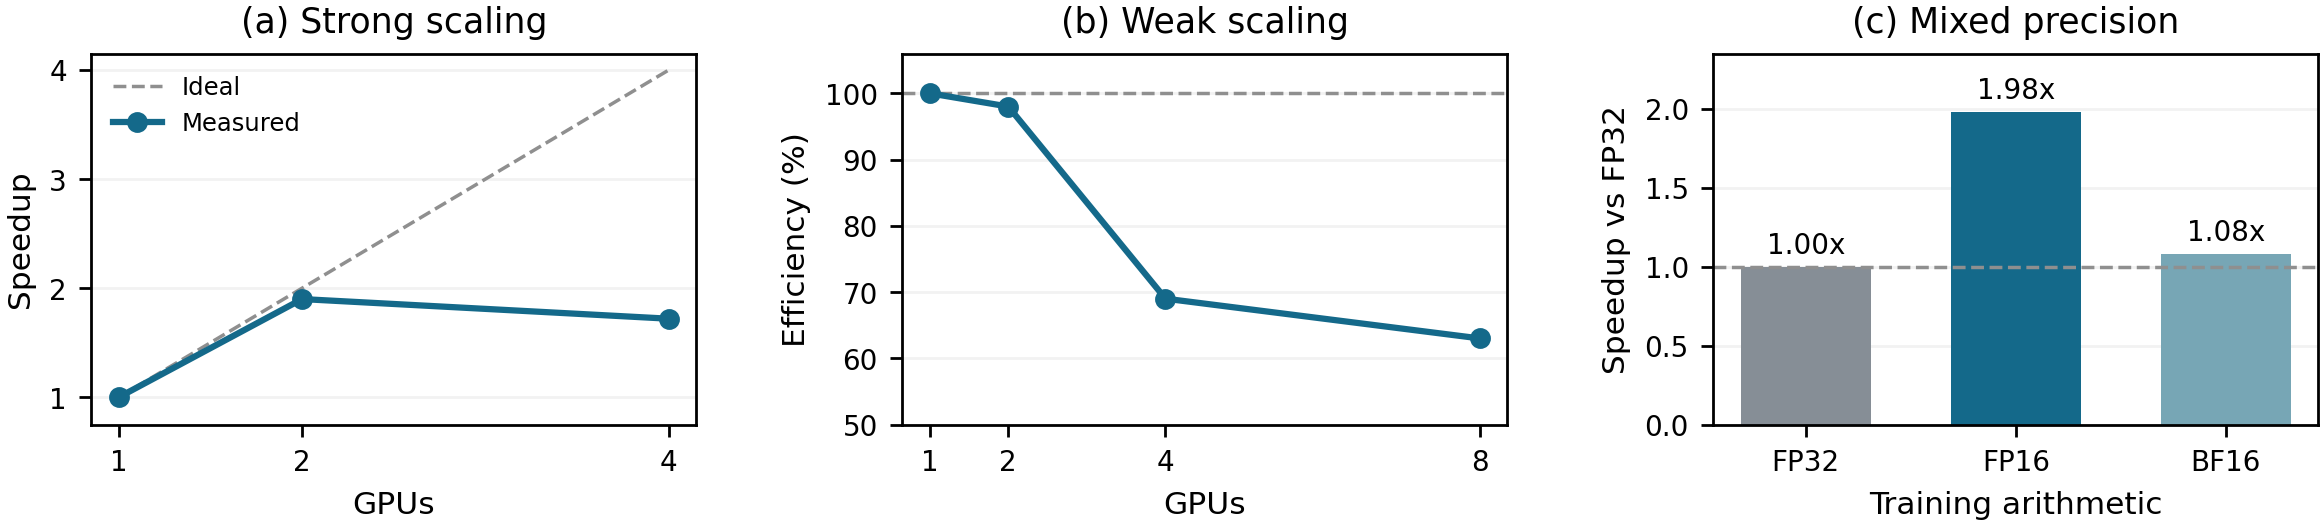
\includegraphics[width=1\linewidth]{ADASS26_C202_f2.png}
\caption{Leonardo GPU benchmarks: (a) strong-scaling speedup,
(b) weak-scaling efficiency and (c) mixed-precision FP16 and BF16
speedup relative to FP32. Dashed lines indicate ideal or baseline
performance. Error bars represent the standard deviation over four
repeated runs.}
\label{fig:performance}
\end{figure}

\begin{table}[!ht]
\caption{Test-set segmentation metrics (mean $\pm$ standard deviation)
for the different training configurations. The single-GPU FP32
run is the common reference. Strong- and weak-scaling runs use FP32.}
\label{tab:tuna_quality}
\smallskip
\begin{center}
{\small
\setlength{\tabcolsep}{5pt}
\begin{tabular}{lcccc}
\tableline
\noalign{\smallskip}
Configuration & IoU & F1 & Recall & Precision \\
\noalign{\smallskip}
\tableline
\noalign{\smallskip}
FP32 baseline (1 GPU) & $0.566\pm0.005$ & $0.720\pm0.004$ & $0.654\pm0.012$ & $0.805\pm0.009$ \\
\noalign{\smallskip}
\tableline
\noalign{\smallskip}
Strong scaling (2 GPUs) & $0.566\pm0.003$ & $0.719\pm0.003$ & $0.653\pm0.004$ & $0.805\pm0.003$ \\
Strong scaling (4 GPUs) & $0.566\pm0.001$ & $0.719\pm0.001$ & $0.653\pm0.009$ & $0.806\pm0.010$ \\
\noalign{\smallskip}
\tableline
\noalign{\smallskip}
Weak scaling (2 GPUs) & $0.566\pm0.001$ & $0.718\pm0.001$ & $0.656\pm0.010$ & $0.801\pm0.014$ \\
Weak scaling (4 GPUs) & $0.564\pm0.002$ & $0.718\pm0.003$ & $0.653\pm0.005$ & $0.803\pm0.004$ \\
Weak scaling (8 GPUs) & $0.564\pm0.002$ & $0.717\pm0.002$ & $0.655\pm0.009$ & $0.799\pm0.011$ \\
\noalign{\smallskip}
\tableline
\noalign{\smallskip}
Mixed FP16 (1 GPU) & $0.566\pm0.002$ & $0.718\pm0.002$ & $0.652\pm0.005$ & $0.805\pm0.009$ \\
Mixed BF16 (1 GPU) & $0.565\pm0.001$ & $0.719\pm0.001$ & $0.652\pm0.004$ & $0.807\pm0.003$ \\
\noalign{\smallskip}
\tableline
\end{tabular}
}
\end{center}
\end{table}

%\subsection{Mixed precision and segmentation quality}

On a single NVIDIA A100 GPU, mixed-precision FP16 training achieved a mean
speedup of $1.98\times$ relative to FP32, whereas mixed-precision BF16
training achieved a mean speedup of $1.08\times$
(Fig.~\ref{fig:performance}c). The BF16 result should be considered
preliminary. Although the A100 provides native BF16 support, its limited
speedup may depend on implementation-specific factors, such as kernel
selection and operations remaining in FP32. Further investigation is required
before drawing general conclusions about BF16 performance.

The segmentation metrics remain remarkably stable across the different GPU configurations and numerical precision formats (see Table \ref{tab:tuna_quality}). Relative to the single-GPU FP32 baseline, the largest absolute differences are 0.002 in IoU and recall, 0.003 in F1, and 0.006 in precision. These variations indicate that neither increasing the number of GPUs nor adopting mixed-precision training introduces substantial degradation in segmentation performance. In particular, the nearly twofold training acceleration obtained with FP16 is accompanied by essentially unchanged segmentation quality.

\section{Conclusions}

TUNA enables survey-scale segmentation of extended radio galaxies
and diffuse cluster emission. FP16
substantially reduced training time without an observable degradation in segmentation quality, while the BF16 performance result remains
preliminary. Strong-scaling saturation
made the allocation of additional GPUs increasingly inefficient. Future work will target
LoTSS-DR3 and multimodal source classification. Evaluating time to solution
and scientific quality together is key to resource-efficient survey analysis.



\acknowledgements This paper has been supported by the Fondazione ICSC, Spoke 3 Astrophysics and Cosmos Observations. National Recovery and Resilience Plan (PNRR) Project ID CN\_00000013 "Italian Research Center for High-Performance Computing, Big Data and Quantum Computing". We acknowledge the CINECA award under the ISCRA programme project IscrC\_SNILV.


\bibliography{c202}  % For BibTex


\end{document}
